\documentclass{beamer}

\usepackage{graphicx}
\usepackage{xcolor}

\title{Let's find your new home!\\ Eau Claire, Wisconsin}
\author{Eric Canton}
\date{}

\mode<presentation>
{
    \usetheme{Hannover}
}

\begin{document}

\begin{frame}
    \maketitle
\end{frame}

\section{Eau Claire: Overview}
\begin{frame}
    \begin{itemize}
        \item Eau Claire is a small city in west-central Wisconsin with an estimated 2018 population of about 69,000 within city limits, and about 160,000 in the metropolitan area.\pause
    
        \item In addition to a vibrant downtown area around the University of Wisconsin campus, there are many parks and schools scattered throughout and surrounding the city. 

    \pause
        \item To help narrow your search, we analyzed 54 houses for sale on Trulia.com, based on Foursquare venues.\pause
            
        \item 
            The features of these listings we focused on include:
            \begin{enumerate}
                \item Total density of shops, restaurants, and other venues within 750 meters (0.47 miles) of a listing. \pause
                \item Number of coffee shops, schools, libraries, bookstores, and parks/playgrounds within 2400 meters (1.5 miles).
            \end{enumerate}
            Let's take a look at what we found!
    \end{itemize}
\end{frame}

\section{Total Density}
\begin{frame}
    \begin{itemize}
        \item Even the densest neighborhoods with houses for sale are not too dense. No listing we investigated had more than 36 venues within a 750 meter radius. \pause
        \item Using an automated process ($K$-means clustering) we grouped houses into low, medium, and high densities.\pause 
            In terms of number of venues, these translated to:
            \begin{itemize}
                \item[$\star$] Low: 9 or fewer venues (within 750 meters)
                \item[$\star$] Medium: 11 to 18 venues
                \item[$\star$] High: 23 to 36 venues \pause
            \end{itemize}
            
        \item On the next slide, we have plotted the listings color-coded by density: 
            (low/green), (medium/yellow), (high/red).
%        \item On the next slides, we have plotted and mapped the densities. Our plot includes the break points for low/medium/high density, to give some feel for how the densities are distributed. The map indicates these as  \pause
%        \item Our company standard is to measure density out of 50 venues. 
    \end{itemize}
\end{frame}

%\subsection{Graph}
%\begin{frame}
%    %\begin{center} 
%     Density : (\# venues within 750m)/50
%    \vspace{-0.55cm}
%    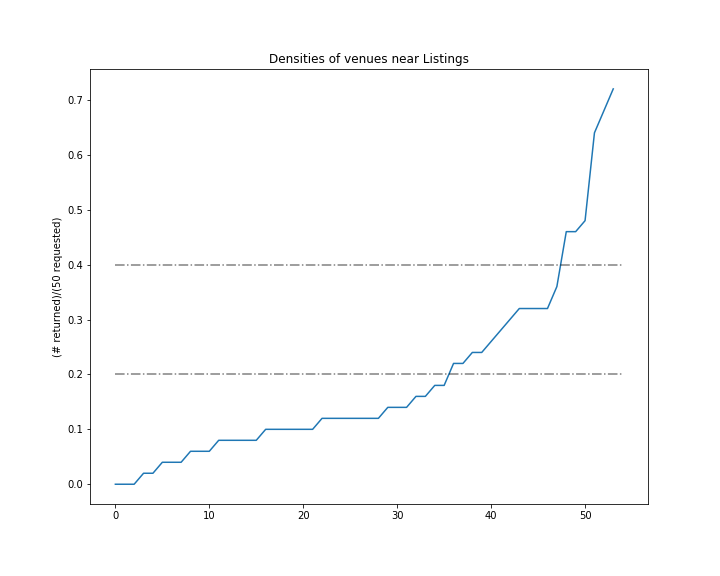
\includegraphics[scale=0.45]{Densities_plot.png}
%    %\end{center}
%\end{frame}
%
\subsection{Map}
\begin{frame}
    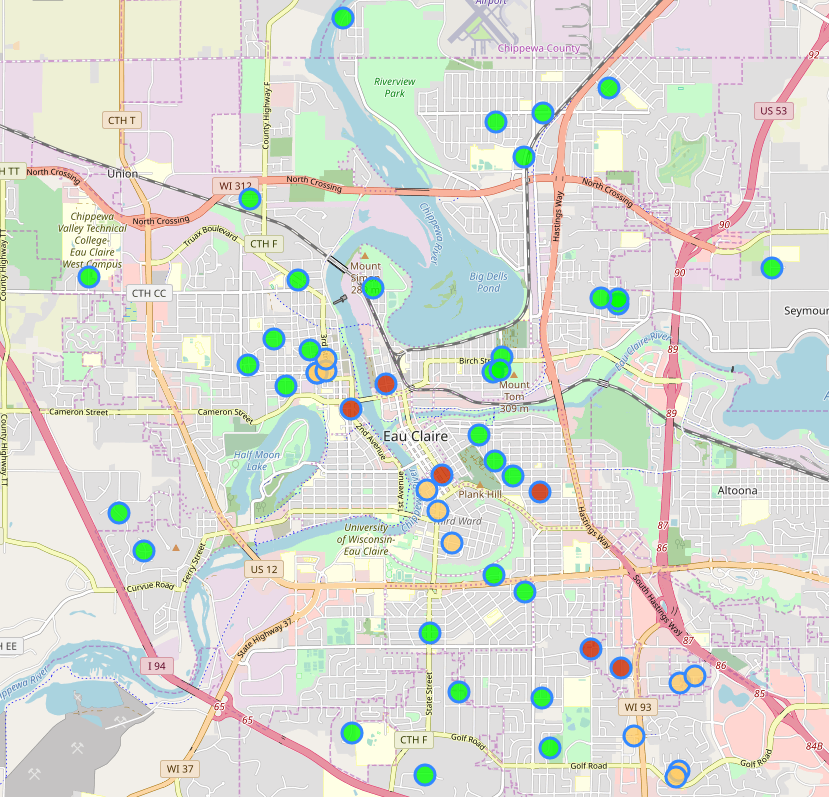
\includegraphics[scale=0.45]{Densities.png}
\end{frame}

\section{Schools, Coffee, etc.}
\subsection{OPTICS}
\begin{frame}
    We used a second automatic clustering tool, called OPTICS, to find natural groupings of houses for sale based on the number of venues of special interest you discussed prior to our investigation. These categories were:
    \begin{itemize}
        \item Coffee shops
        \item Schools (pre/elementary/middle/high)
        \item Libraries
        \item Bookstores
        \item Parks/playgrounds
    \end{itemize}
\end{frame}

\begin{frame}
    \begin{itemize}
        \item OPTICS found five main clusters of homes, in addition to a number of houses that did not fit into the natural clusters discovered. \pause

        \item On the next slide, we have plotted the average number of venues of each category within 1.5 miles of the house listings. \pause
            
        \item A key distinguishing feaure between clusters 0 and 1, versus 2 through 4, is the number of parks nearby. \pause

        \item We included averages for the outliers; since these houses are somewhat dissimilar and spread around Eau Claire, one might interpret these averages as general/city-wide. 
    \end{itemize}
\end{frame}

\subsection{Averages per cluster}
\begin{frame}
    %\begin{center}
    \hspace{-0.6cm}
    \begin{minipage}{\textwidth}
    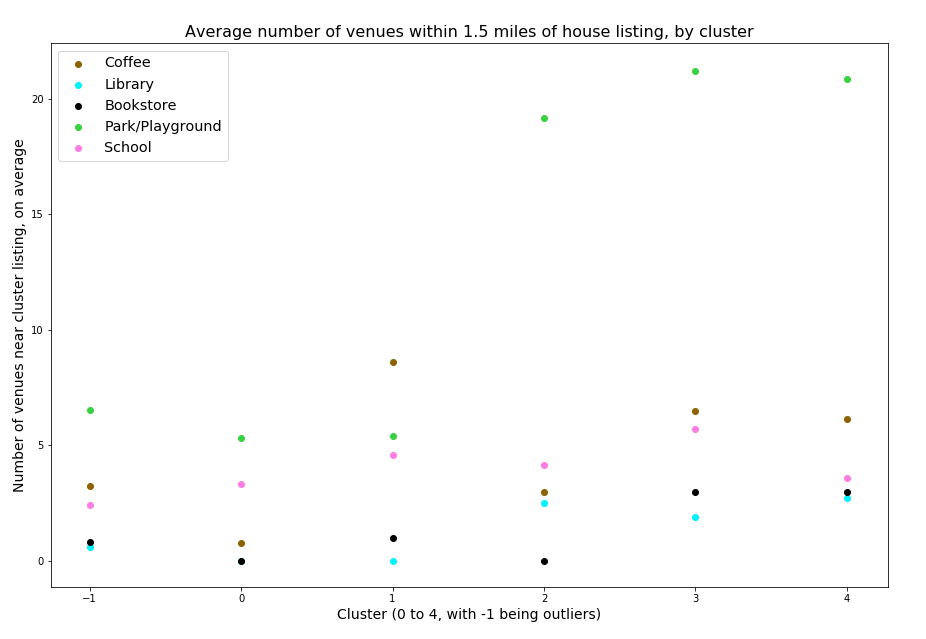
\includegraphics[scale=0.35]{Avg_venues.png}
    \end{minipage}\hspace{5cm}
    %\end{center}
\end{frame}

\subsection{Map}
\begin{frame}
    \begin{center}
        \vspace{-0.5cm}
        \hspace{-1.25cm}
        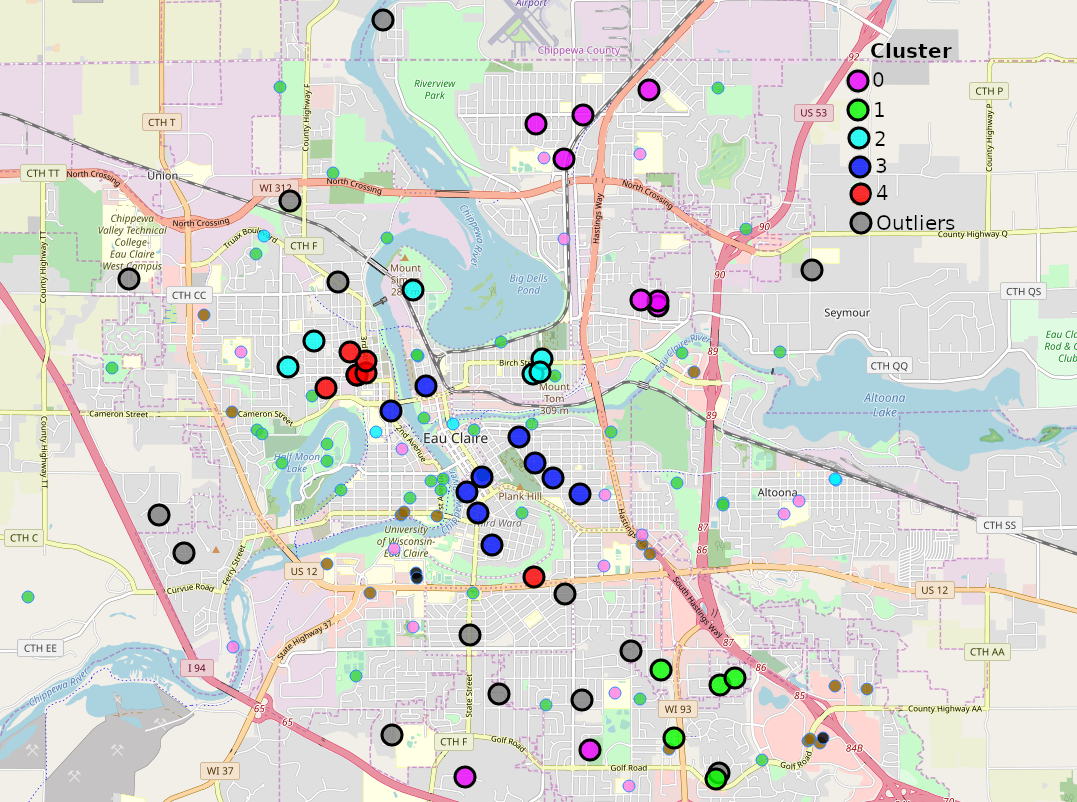
\includegraphics[scale=0.42]{Clusters.png}
        \vspace{1cm}
    \end{center}
\end{frame}

\subsection{Recommendations}
\begin{frame}
    \begin{itemize}
        \item Cluster 1 has more coffee shops nearby than any other, on average, but is close to several highways and a mall, so many of the shops are chains. \pause
        \item Cluster 3 has many nearby parks, as well as many coffee shops and schools. 
        \item Cluster is downtown or adjacent-to-downtown, close to the {\em Third Ward} neighborhood.
        \item  Our professional contacts in the academic departments of University of Wisconsin indicate this is a popular choice of neighborhood for professors. 
    \end{itemize}
\end{frame}

\subsection{Next steps}
\begin{frame}
    \begin{itemize}
        \item We are happy to continue providing comparative and clustering analysis of new listings. \pause
        \item Once you have decided on region(s) in Eau Claire that interests you, we can also help with comparative analysis of homes in the region(s).
    \end{itemize}
\end{frame}

\begin{frame}
    We will provide you with interactive versions of the maps from this presentation, along with finer-detailed analysis of the listings.
\end{frame}


\begin{frame}
    \begin{center}
        Thank you for consulting with us!
    \end{center}
\end{frame}

\end{document}
